% -*- coding: UTF-8 -*-
% gougu.tex
% 勾股定理
\documentclass[UTF8]{ctexart}
\usepackage{graphicx}
\usepackage{float}
\usepackage{amsmath}

\usepackage{geometry}
\geometry{a6paper,centering,scale=0.8}

\usepackage[format=hang, font=small, textfont=it]{caption}

\usepackage[nottoc]{tocbibind}

\newcommand{\degree}{^\circ}

\title{\heiti 杂谈勾股定理}
\author{\kaishu 张三}
\date{\today}

\bibliographystyle{plain}

\newtheorem{thm}{定理}

\newenvironment{myquote}
{ \begin{quote} \kaishu \zihao{-5} }
{ \end{quote} }

\begin{document}

\maketitle

\begin{abstract}
    这是一篇关于勾股定理的小短文。
\end{abstract}

\tableofcontents
\section{勾股定理在古代}\label{sec:1}
西方称勾股定理为毕达哥拉斯定理,将勾股定理的发现归功于公元前 6 世纪的毕达哥拉斯学派\cite{Kline}。该学派得到了一个法则,可以求出可排成直角三角形三边的三元组。毕达哥拉斯学派没有书面著作,该定理的严格表述和证明则见于欧几里得\footnote{欧几里得,约公元前330--275年。}《几何原本》的命题 47:“直角三角形斜边上的正方形等于两直角边上的正方形之和。”证明是用面积做的。


我国《周髀算经》载商高(约公元前 12 世纪)答周工问:
\begin{myquote}
    勾广三,股修四,径隅五。
\end{myquote}
又载陈子(约公元前 7--6 世纪)答荣方问:
\begin{myquote}
    若求邪至日者,以日下为勾,日高为股,勾股各自乘,并而开方除之,得邪至日。
\end{myquote}
都较希腊较早。后者已经明确道出勾股定理的一般形式。图\ref{fig:xiantu}是我国古代对勾股定理的一种证明\cite{quanjing}。

\begin{figure}[ht]
    \centering
    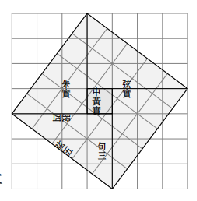
\includegraphics[scale=0.8]{xiantu.pdf}
    \caption{宋赵爽在《周髀算经》注中作的弦图(仿制),该图给出了勾股定理的一个极具对称美的证明。}
    \label{fig:xiantu}
\end{figure}

\section{勾股定理的近代形式}

勾股定理可以用现代语言表述如下:

\begin{thm}[勾股定理]
    直角三角形斜边的平方等于两腰的平方和。

    可以用符号语言表述为:设直角三角形 ABC ,其中$C=90\degree$,则有
    \begin{equation}\label{eq:gougu}
        AB^2 = BC^2 + AC^2 
    \end{equation}
\end{thm}


满足式\eqref{eq:gougu}的整数称为\emph{勾股数}。第 \ref{sec:1} 节所说毕达哥拉斯学派得到的三元数组就是勾股数。下面列出一些较小的勾股数:

\begin{table}[H]
    \begin{tabular}{|rrr|}
        \hline
        直角边 $a$ & 直角边 $b$ & 斜边 $c$ \\ 
        \hline
        3 & 4 & 5 \\ 
        5 & 12 & 13 \\ 
        \hline
    \end{tabular}%
    \qquad
    ($a^2 + b^2 = c^2$)
\end{table}

\nocite{Shiye}
\bibliography{math}

\end{document}